%%%%%%%%%%%%%%%%%%%%%%%%%%%%%%%%%%%%%%
% This is the name of the style file.
%%%%%%%%%%%%%%%%%%%%%%%%%%%%%%%%%%%%%%
%
% phd  -> for a PhD dissertation
% ms   -> for an MS thesis
% If both phd and ms are used then phd will overide.  If none are used,
% then ms will be active by default.
%
% cpyr -> generate a copyright page
% lof  -> generate List of Figures
% lot  -> generate List of Tables
\documentclass[ms,cpyr,lof,lot]{uathesis}
%
%%%%%%%%%%%%%%%%%%%%%%%%%%%%%%%%
% List of any packages you use.
%%%%%%%%%%%%%%%%%%%%%%%%%%%%%%%%
%

%% FROM REU SUMMARY


\usepackage{graphicx}
\usepackage{amsmath,amssymb}
%\usepackage{gensymb}
\usepackage{mathtools}
\usepackage{etoolbox}
\usepackage{booktabs}
\usepackage{float}
\usepackage{graphicx}
\usepackage{geometry}
\usepackage{multicol}
\usepackage{caption}
\usepackage[outdir=./eps2pdf/]{epstopdf}
\graphicspath{
  {figures/}
  {figures/goals/}
  {figures/light_data/}
  {figures/attenuation/}
}

%%%%%%%%%%%%%%%%%%%%%%%%%%%%%%%%%%
% List of definitions you define.
%%%%%%%%%%%%%%%%%%%%%%%%%%%%%%%%%%


\DeclareMathOperator{\atantwo}{atan2}


%% FROM GOALS
\newcommand\plotwidth{7in}

%% FROM REU SUMMARY

\newcommand{\ds}{\displaystyle}

% Define error function for math mode
\newcommand{\erf}{\mbox{erf}}
% Sign function
\newcommand{\sign}{\mbox{sign}}
% Real numbers
\newcommand\R{\mathbb{R}}
% Norm
\newcommand\norm[1]{||#1||}
% Length matrix entries
\newcommand\LL{\mathcal{L}}
% Frond population
\newcommand\FF{\mathcal{F}}

%% FROM RTE PAPER

% Natural numbers
\newcommand\NN{\mathbb{N}}
% Real numbers
\newcommand\RR{\mathbb{R}}
% Complex numbers
\newcommand\CC{\mathbb{C}}
% Curly B for basis
\newcommand\BB{\mathcal{B}}
% Curly D for diagonal dominance quantity
\newcommand\DD{\mathcal{D}}
\newcommand\QQ{\mathcal{Q}}
% Uniform Norm
\newcommand\unorm[1]{\left\lVert #1 \right\rVert_\infty}
% Inner Product
\newcommand\ip[1]{\left\langle #1 \right\rangle}
% Absolute value
\newcommand\abs[1]{\left| #1 \right|}
% Complex Conjugate
\newcommand\conj\overline
% Partial derivative
\newcommand\pd[2]{\frac{\partial #1}{\partial #2}}
% Iteration superscript w/ parentheses
\newcommand{\iter}[1]{^{(#1)}}
% Disable paragraph indentation
%\setlength{\parindent}{0pt}
% End of proof
\newcommand\qed{\hfill$\blacksquare$\hspace{0.5in}}


\title{Modelling the Radiation Field in Macroalgae Aquaculture}
\author{Oliver Graham Evans}
\conferraldate{May}{2018}

%The following commands specify the names and titles of people that
%will appear on the signature page.
%
%These four will always be needed.
\advisor{Dr. Kevin Kreider}
\chair{Dr. Kevin Kreider}
\collegedean{Dr. John Green}
\gradschdean{Dr. Chand Midha}
%
%For a PhD dissertation, specify a coadvisor and three committee
%members, or four committee members only.  For an MS thesis use either
%one coadvisor or one faculty reader, not both.
%
%Typical commands for a PhD dissertation (uncomment only 4).
%\coadvisor{Name of Coadvisor}
%\committee{Name of 1st Comm Member}
%\committee{Name of 2nd Comm Member}
%\committee{Name of 3rd Comm Member}
%\committee{Name of 4th Comm Member}
%
%Typical commands for an MS thesis (uncomment only 1).
\coadvisor{Dr. Curtis Clemons}
%\facreader{Name of Fac Reader}
%\facreader{Name of Fac Reader}

\begin{document}

\maketitle
\chapter{INTRODUCTION} \label{ch:intro}

\section{Purpose, Kelp \& WWTPs}
I spent this summer participating in an REU at Clarkson University developing a mathematical model for the light field in a macroalgae aquaculture environment. The impetus for this project was as follows: Dr. Rogers was approached by the operator of a wastewater treatment plant in Boothbay Harbor, Maine, who is facing increasingly demanding EPA regulations limiting the concentration of certain nutrients permissible to be released into the ocean via wastewater treatment outfalls.
In order to adhere to these stricter requirements using conventional nutrient remediation, a significant quantity of specialized equipment would be necessary, which is not currently present in the Boothbay Harbor plant.
Being surrounded on all sides by water and private property, the treatment plant lacks the necessary space for the additional equipment, and would therefore need to move their entire facility to a new location in order to conform to these new nutrient regulations.

As an alternative to conventional nutrient remediation techniques, Dr. Rogers has proposed the cultivation of the macroalgae \textit{Saccharina Latissima} (sugar kelp) near the outfall site.
The purpose of such an undertaking would be twofold: to prevent eutrophication of the surrounding ecosystem by sequestering the nutrients in question, and to reduce one of the primary expenses in macroalgae cultivation: nutrient input.
Once grown, a variety of products can be derived from macroalgae, including biofuel, fish/cattle feedstock, and high value chemical materials such as alginate and agar.
Food for human consumption is also a common product of kelp aquaculture, though it may not be ideal for a wastewater treatment application.

Thus, we seek to investigate the feasibility, and optimal implementation of kelp farming in wastewater treatment operations. 
Specifically, I seek to develop an accurate model of the light field in a kelp farming environment as a function of both the spacing and depth of the kelp plants, and of the quality of the water itself.
Ole Jacob Broch is a mathematician at SINTEF, a research organization in Trondheim, Norway, who has been working to model the growth of \textit{Saccharina Latissima} using SINMOD, a large-scale 3D hydrodynamical ocean model developed at SINTEF.
Ultimately, my aim is that my light model can be used both independently and in conjunction with Dr. Broch's SINMOD model.

\section{Background on Kelp Models}

Mathematical modeling of macroalgae growth is not a new topic, although it is a reemerging one.
Several authors in the second half of the twentieth century were interested in describing the growth and composition of the macroalgae \textit{Macrocystis pyrifera}, commonly known as ``giant kelp,'' which grows prolifically off the coast of southern California.
The very first such mathematical model was developed by W.J. North for the Kelp Habitat Improvement Project at the California Institute of Technology in 1968 using seven variables.
By 1974, Nick Anderson greatly expanded on North's work, and created the first comprehensive model of kelp growth which he programmed using FORTRAN \cite{anderson_mathematical_1974}.
In his model, he accounts for solar radiation intensity as a function of time of year and time of day, and refraction on the surface of the water.
He uses a simple model for shading, simply specifying a single parameter which determines the percentage of light which is allowed to pass through the kelp canopy floating on the surface of the water.
He also accounts for attenuation due to turbidity using Beer's Law.
Using this data on the availability of light, he calculates the photosynthesis rates and the growth experienced by the kelp. \\[-0.75em]

Over a decade later in 1987, G.A.
Jackson expanded on Anderson's model for \textit{Macrocystis pyrifera}, with an emphasis on including more environmental parameters and a more complete description of the growth and decay of the kelp \cite{jackson_modelling_1987}. 
He takes into account respiration, frond decay, and most importantly for my work, sub-canopy light attenuation due to self-shading.
He simply adds a coefficient to the exponential decay of light as a function of depth to represent shading from kelp fronds.
He doesn't seem to consider and radial nor angular dependence on shading.
Jackson also expands Anderson's definition of canopy shading, treating the canopy not as a single layer, but as 0, 1, or 2 discrete layers, each composed of individual fronds.
While this is a significant improvement over Anderson's light model, it is still rather simplistic. \\[-0.75em]

Both Anderson's and Jackson's model were carried out by numerically solving a system of differential equations over small time intervals.
In 1990, M.A. Burgman and V.A. Gerard developed a stochastic population model \cite{burgman_stage-structured_1990}.
This approach is quite different, and functions by dividing kelp plants into groups based on size and age, and generating random numbers to determine how the population distribution over these groups changes over time, based on measured rates of growth, death, decay, light availability, etc.
That same year, Nyman et. al. tested a similar model in New Zealand, as well as a Markov chain model, and compared the results with experimental data \cite{nyman_macrocystis_1990}. \\[-0.75em]

In 1996 and 1998 respectively, P. Duarte and J.G. Ferreira used the size-class approach to create a more general model of macroalgae growth, and Yoshimori et. al. created a differential equation model of \textit{Laminaria religiosa} with specific emphasis on temperature dependence of growth rate \cite{duarte_model_1996,yoshimori_mathematical_1998}.
These were the some of the first models of kelp growth that did not specifically relate to \textit{Macrocystis pyrifera} (``giant kelp''). 
Initially, there was a great deal of excitement about this species due to it's incredible size and growth rate, but difficulties in harvesting and negative environmental impacts have caused scientists to investigate other kelp species. \\[-0.75em]

In the last five years, a team at SINTEF, a research organization associated with the Norwegian University of Technology and Science (NTNU), based in Trondheim, Norway, has become interested in the aquaculture potential of the kelp \textit{Saccharina latissima} for use as food, animal feed, nutrient remediation, biofuel production, and high-value chemical production among other uses. 
In 2012, Ole Jacob Broch, whom I have been working with for the last few weeks, published a paper with Dag Slagstad describing the model they created of the growth and composition of \textit{S. latissima} over the course of the year \cite{broch_modelling_2012}.
Their model works in conjunction with SINMOD, a 3D hydrodynamic ecosystem model developed at SINTEF which generates data on water temperature, water velocity, light intensity, and phytoplankton concentrations among other valuable quantities \cite{wassmann_modelling_2006}.
This detailed information has allowed Ole Jacob to consider many factors which influence the growth and decay of kelp in greater detail than has previously been explored. \\[-0.75em]

The aspect of the model that he has asked me to help develop is how light is attenuated by kelp plants and by environmental factors, and how that affects the kelp's ability to photosynthesize and grow. 
This will allow us to estimate how deep and how densely kelp can be grown. This work is being done as a part of the MacroSea project, funded by the Norwegian Research Council, which intends to further develop the potential industrial kelp production through collaboration among industry and academia both in Norway and abroad. SINTEF and Clarkson are both involved in the project. \\[-0.75em]

In my model, I intend to combine the probabilistic aspects of models such as the one developed by \cite{burgman_stage-structured_1990} with numerically solving a system of differential equations such as is done by \cite{anderson_mathematical_1974} and \cite{broch_modelling_2012}
For example, the concept of a Lefkovitch model, which is essentially a Markov chain model which describes the change size distribution of a biological population which is broken up into discreet size classes, may prove to be very useful \cite{caswell_matrix_1983}. Combining the idea of a probabilistic model of shading based on the distribution of frond lengths and angles with differential equations describing the growth and decay of kelp fronds as a function of light availability may prove to be very powerful. I intend to analyze experimental data collected here in Norway, as well as in Maine and elsewhere in the literature to verify the model. \\[-0.75em]

\section{Background on Radiative Transfer}

We use monochromatic radiative transfer in order to model the light field in an aqueous environment populated by vegetation.
The vegetation (kelp) is modeled by a spatial probability distribution, which we assume to be given.
The two quantities we seek to compute are \textit{radiance} and \textit{irradiance}.
Radiance is the intensity of light in at a particular point in a particular direction, while irradiance is the total light intensity at a point in space, integrated over all angles.
The Radiative Transfer Equation is an integro-partial differential equation for radiance, which has been used primarily in stellar astrophysics; it's application to marine biology is fairly recent \cite{mobley_radiative_2001}.

We study various methods for solving the system of linear equations resulting from discretizing the Radiative Transfer Equation.
In particular, we consider direct methods, stationary iterative methods, and nonstationary iterative methods.
Numerical experiments are performed using Python's \texttt{scipy.sparse} \cite{jones_scipy:_2001} package for sparse linear algebra.
\texttt{IPython} \cite{perez_ipython:_2007} was used for interactive numerical experimentation.

Among those implemented, the nonstationary \texttt{LGMRES} \cite{baker_technique_2005} algorithm is the only algorithm determined to be suitable for this application without further work.
We discuss limitations and potential improvements, including preconditioning, alternative discretization, and reformulation of the RTE.

Understanding the growth rate and nutrient recovery by
kelp cultures has important marine biological implications. For example, recent
work by our research group at Clarkson University, the University of Maine, and
SINTEF Fisheries and Aquaculture is investigating kelp aquaculture as a means to
recover nutrients from wastewater effluent plumes in coastal environments into a
valuable biomass feedstock for many products. Current models for kelp growth
place little emphasis on the way in which nearby plants shade one another.
Self-shading may be a significant model feature, though, as light availability
may impact the growth and composition of the kelp biomass, and thus the mixture
of goods that may be derived.

\section{Summary of Main Results}
\chapter{THE TWO DIMENSIONAL WAVE EQUATION} \label{2DWaveEquation}

Here is an example of a 'section' and a few equations.

\section{Recurrence Relation}

A series solution for the two-dimensional wave equation
\begin{equation}
\frac{1}{c^{2}}\frac{\partial^{2}u}{\partial t^{2}} = \frac{\partial^{2}u}{\partial r^{2}} + %
        \frac{1}{r}\frac{\partial u}{\partial r} + \frac{1}{r^{2}}\frac{\partial^{2}u}%
        {\partial\theta^{2}}                                                                 \label{waveEq}
\end{equation}
for outgoing waves is
\begin{equation}
u = \sum_{n=0}^{\infty}a_{n}(\theta)f^{n}(r,t),                                              \label{Soln}
\end{equation}
where
\begin{equation}
f^{n} = \sum_{k=0}^{\infty}r^{-k-\frac{1}{2}}f_{k}^{n}(ct-r).                                \label{function}
\end{equation} %look up reference.

You can reference a labeled equation by using the \textit{ref}
command.  For example, you can show that equations (\ref{Soln}) and
(\ref{function}) are a solution to equation (\ref{waveEq}).  (see the
file chap2.tex for the commands).

\section{Second Section Long Subtitle Second Section Long Subtitle Second Section Long Subtitle}
The text for the second section.  The text for the second section.
The text for the second section.  The text for the second section.
The text for the second section.  The text for the second section.
The text for the second section.  The text for the second section.

\subsection{First Subsection}
The text for the first subsection of the second section.  The text for
the first subsection of the second section.  The text for the first
subsection of the second section.  The text for the first subsection
of the second section.  The text for the first subsection of the
second section.  The text for the first subsection of the second
section.  The text for the first subsection of the second section.
The text for the first subsection of the second section.

\section{Third Section}
The text for the third section.  The text for the third section.  The
text for the third section.  The text for the third section.  The text
for the third section.  The text for the third section.  The text for
the third section.  The text for the third section.

\chapter{MODEL ANALYSIS} \label{ch:model_analysis}

\section{Kelp Model}
\subsection{Grid Study}
Run many grid sizes with GMRES, using asymptotic solution as initial guess.
Compare CPU time and accuracy. Determine necessary 

\subsection{Parameter Study}

\section{Light Model}

\subsection{Asymptotics vs. Finite Difference}
\chapter{EXAMPLE OF A TABLE AND A FIGURE} \label{TabAndFigChap}

\begin{table}[h]
\begin{center}
\caption{Table captions belong above the table.  Just some text to lengthen the title of the table beyond a single line.} \label{tb:disc}
\vskip .1 truein
\begin{tabular}{|l||c||c||c|} \hline \hline
\textbf{Name} & \textbf{Variable} & \textbf{Discretization} & \textbf{Step} \\ \hline
Radius      &       $r\in[a,R]$      &          $r_{k} =a + k dr,\quad k=0,1,2,\dots,K$   &    $dr = (R-a)/K$  \\ \hline
Angle       &       $\theta\in[0,2\pi)$ &      $\theta_{l} = l d\theta, \quad l =0,1,2,\dots,L-1$ & $d\theta = 2\pi/L$ \\ \hline
Time         &       $t\in[0,T]$           &      $t_{p} = p dt, \quad p =0,1,2,\dots,P$     &     $dt = T/P$ \\ \hline \hline
\end{tabular}
\end{center}
\end{table}

\begin{figure}[h]
\begin{center}
\includegraphics[width=3in,angle=-90]{Waves.eps}
\end{center}
\caption{Figure labels go below the figure.  Just some text to lengthen the title of the figure beyond a single line.  Just some text to lengthen the title of the figure beyond a single line.} \label{fg:N5Wave}
\end{figure}

To include figures side-by-side use the minipage environment.

\begin{figure}[ht]
\begin{minipage}{0.45\linewidth}
\begin{center}
\includegraphics[width=2.25in,angle=-90]{Waves.eps}
\vspace{0in}\ref{sbys}A:
\end{center}
\end{minipage} \hfill
\begin{minipage}{0.45\linewidth}
\begin{center}
\includegraphics[width=2.25in,angle=-90]{Waves.eps}
\vspace{0in}\ref{sbys}B:
\end{center}
\end{minipage}

%short caption
\caption{Figures side-by side\newline (a) part a (b) part b}\label{sbys}

%long caption (this works)
%\caption{Figures side-by side\newline (a) part a  part a part a part a part a part a part a part a part a part a (b) part b part b part b part b part b part b part b part b part b part b part b part b part b part b part b}\label{sbys}
\end{figure}

See chap4.tex for the commands used to build the table and figure.  As
you add chapters, figures, and tables, the table of contents and lists
will automatically be updated.

Figure~\ref{sbys} is an example of figures side-by-side, with
Figure~\ref{sbys}A to the left of \ref{sbys}B.

\section{First Section}
The text for the first section.  The text for the first section.  The
text for the first section.  The text for the first section.  The text
for the first section.  The text for the first section.  The text for
the first section.  The text for the first section.

\section{Second Section}
The text for the second section.  The text for the second section.
The text for the second section.  The text for the second section.
The text for the second section.  The text for the second section.
The text for the second section.  The text for the second section.

\subsection{First Subsection}
The text for the first subsection of the second section.  The text for
the first subsection of the second section.  The text for the first
subsection of the second section.  The text for the first subsection
of the second section.  The text for the first subsection of the
second section.  The text for the first subsection of the second
section.  The text for the first subsection of the second section.
The text for the first subsection of the second section.

\section{Third Section}
The text for the third section.  The text for the third section.  The
text for the third section.  The text for the third section.  The text
for the third section.  The text for the third section.  The text for
the third section.  The text for the third section.

\section{Forth Section}
The text for the forth section.

%%% Local Variables: 
%%% mode: latex
%%% TeX-master: t
%%% End: 

\chapter{NUMERICS}
\section{Numerical Methods}

\section{Simulation Results}
\chapter{CONCLUSION}
\bibliographystyle{unsrt}
\bibliography{bio}
%If you have n appendices, then use the \appendices{n} command below
%followed by n \input{filename} commands, similar to the \input{chapx}
%commands above.
% DO NOT USE SECTIONS OR SUBSECTIONS IN AN APPENDIX OR APPENDICES
% \appendix{3}
% \chapter{APPENDIX TITLE GOES HERE} \label{ap:a}


{\bf DO NOT SECTION OR SUBSECTION AN APPENDIX OR APPENDICS}

We will recylcle Chapters~\ref{2DWaveEquation} and \ref{TabAndFigChap}
to make the following two appendices.


%%%%%%% DO NOT SECTION APPENDICES





% \chapter{SECOND APPENDIX: THE TWO DIMENSIONAL WAVE EQUATION} \label{ap:2DWaveEquation}

{\bf  DO NOT SECTION OR SUBSECTION AN APPENDIX OR APPENDICES}

A series solution for the two-dimensional wave equation
\begin{equation}
\frac{1}{c^{2}}\frac{\partial^{2}u}{\partial t^{2}} = \frac{\partial^{2}u}{\partial r^{2}} + %
        \frac{1}{r}\frac{\partial u}{\partial r} + \frac{1}{r^{2}}\frac{\partial^{2}u}%
        {\partial\theta^{2}}                                                                 \label{ap:waveEq}
\end{equation}
for outgoing waves is
\begin{equation}
u = \sum_{n=0}^{\infty}a_{n}(\theta)f^{n}(r,t),                                              \label{ap:Soln}
\end{equation}
where
\begin{equation}
f^{n} = \sum_{k=0}^{\infty}r^{-k-\frac{1}{2}}f_{k}^{n}(ct-r).                                \label{ap:function}
\end{equation} %look up reference.

You can reference a labeled equation by using the \textit{ref}
command.  For example, you can show that equations (\ref{ap:Soln}) and
(\ref{ap:function}) are a solution to equation (\ref{ap:waveEq}).
(see the file chap2.tex for the commands).



% \chapter{EXAMPLE OF A TABLE AND A FIGURE} \label{ap:TabAndFigChap}

{\bf DO NOT SECTION OR SUBSECTION AN APPENDIX OR APPENDICES}

\begin{table}[h]
\begin{center}
\caption{Table captions belong above the table} \label{ap:tb:disc}
\vskip .1 truein
\begin{tabular}{|l||c||c||c|} \hline \hline
\textbf{Name} & \textbf{Variable} & \textbf{Discretization} & \textbf{Step} \\ \hline
Radius      &       $r\in[a,R]$      &          $r_{k} =a + k dr,\quad k=0,1,2,\dots,K$   &    $dr = (R-a)/K$  \\ \hline
Angle       &       $\theta\in[0,2\pi)$ &      $\theta_{l} = l d\theta, \quad l =0,1,2,\dots,L-1$ & $d\theta = 2\pi/L$ \\ \hline
Time         &       $t\in[0,T]$           &      $t_{p} = p dt, \quad p =0,1,2,\dots,P$     &     $dt = T/P$ \\ \hline \hline
\end{tabular}
\end{center}
\end{table}

\begin{figure}[h]
\begin{center}
\includegraphics[width=3in,angle=-90]{Waves.eps}
\end{center}
\caption{Figure labels go below the figure} \label{ap:fg:N5Wave}
\end{figure}

To include figures side-by-side use the minipage environment.

\begin{figure}[ht]
\begin{minipage}{0.45\linewidth}
\begin{center}
\includegraphics[width=2.25in,angle=-90]{Waves.eps}
\vspace{0in}\ref{ap:sbys}A:
\end{center}
\end{minipage} \hfill
\begin{minipage}{0.45\linewidth}
\begin{center}
\includegraphics[width=2.25in,angle=-90]{Waves.eps}
\vspace{0in}\ref{ap:sbys}B:
\end{center}
\end{minipage}
\caption{Figures side-by side}\label{ap:sbys}
\end{figure}

See chap4.tex for the commands used to build the table and figure.  As
you add chapters, figures, and tables, the table of contents and lists
will automatically be updated.

Figure~\ref{ap:sbys} is an example of figures side-by-side, with
Figure~\ref{ap:sbys}A to the left of \ref{ap:sbys}B.


\end{document}
